\documentclass[10pt,twocolumn]{article}

\usepackage[a4paper,margin=18mm]{geometry}
\usepackage{amsmath,amssymb}
\usepackage{booktabs}
\usepackage{graphicx}
\usepackage{microtype}
\usepackage{siunitx}
\usepackage{caption}
\usepackage{url}
\usepackage[hidelinks]{hyperref}
\usepackage{balance}

\sisetup{detect-weight=true,detect-family=true}

\title{\Large\bfseries Lossless Compression of Range--FFT Data for
SoC-Based Cascaded MIMO Radar:\\
Implementation and Verification of DRHE and LPC on a Kintex UltraScale+ FPGA}

\author{Jordan Mohindra\\[2pt]
\small School of Electrical Engineering and Telecommunications\\
\small UNSW Sydney\\
\small \texttt{z5418455}}

\date{September 2026}

\begin{document}
\maketitle

\begin{abstract}
\noindent
Cascaded millimetre-wave MIMO radar produces range--FFT data faster than a
typical SoC can move it to memory, so a lossless compressor placed between the
FFT and the memory bus is an attractive way to buy back bandwidth. This paper
implements, verifies and critically evaluates two such compressors on real
data: Doppler Redundancy Hybrid Encoding (DRHE), a streaming polar-domain IIR
predictor, and a second-order linear predictive coder (LPC) with Yule--Walker
coefficients. Both share an S4 + APPEND + fixed-Huffman entropy back end. Both
were implemented in Vitis HLS for an AMD Kintex UltraScale+ \texttt{xcku5p},
verified bit-exactly against a MATLAB golden reference over 50 frames of the
ColoRadar cascade dataset, and characterised through RTL co-simulation.

Three findings are reported that change how the results should be read. First,
the headline compression ratio is dominated not by prediction but by the
entropy coder operating on an under-filled 16-bit container: coding the
quantised FFT output with no prediction at all already yields
\num{3.489}, against \num{3.319} for DRHE and \num{3.397} for LPC. Second, and
explaining that inversion, both predictors were being applied along the wrong
axis. The ramp index of a 12-transmitter TDM-MIMO cascade interleaves
transmitters, so ``the previous ramp'' is a different physical antenna eleven
times out of twelve. Predicting at lag $n_{\mathrm{Tx}}$ instead of lag 1
converts a \SI{4.9}{\percent} loss into an \SI{8.2}{\percent} gain, lifting
measured DRHE compression from \num{3.310} to \num{3.751} at a cost of
$n_{\mathrm{Tx}}$ copies of the predictor state. Third, the reference
throughput figure of \SI{11.92}{Gbit\per\second} widely quoted for this class of
design is in gibibits per second; in decimal units it is
\SI{12.80}{Gbit\per\second}, exactly \num{128} bits per cycle at
\SI{100}{\mega\hertz}, i.e.\ a full-rate AXI4-Stream at $\mathrm{II}=1$.

Two implementation defects are also documented and fixed: a residual value of
$-32768$ that the S4/APPEND code cannot represent and which silently aliased to
$+32767$, and a 128-bit to single-precision conversion in the Yule--Walker
solver that returned zero for operands above $2^{64}$.
\end{abstract}

\section{Introduction}
\label{sec:intro}

A TI MMWCAS-RF-EVM cascade carries four AWR2243 devices, presenting 16 receive
and 12 transmit channels. At the ColoRadar capture settings used here --- 256
ADC samples per chirp, 16 chirp loops, 12 TDM transmitters --- one frame is
\num{786432} complex samples, or \SI{3}{\mebi\byte} of raw int16 I/Q. The
range--FFT stage halves that (only the positive half-spectrum is retained) but
does not change the order of magnitude. Moving this to DDR every frame period
is the practical bottleneck in an SoC-based radar front end, and it is the
bottleneck a compression IP placed between the FFT output and the memory
interface is meant to relieve.

The compressor must be lossless. Any error introduced before detection
propagates into the CFAR stage, and a radar that silently loses targets to save
bandwidth is not a useful trade. Losslessness also makes verification
unambiguous: the pass criterion is that every reconstructed sample equals its
original exactly, and any nonzero maximum absolute difference is a defect.

This paper has three purposes. The first is to document a complete
implementation and verification flow for two lossless compressors on real
radar data, from a MATLAB golden reference through bit-exact HLS C-simulation
to RTL co-simulation and resource estimation. The second is to audit the
results that flow comes out with --- in particular to ask what the compression
ratio actually measures. The third is to report and fix the defects that audit
exposed.

The remainder is organised as follows. Section~\ref{sec:background} describes
the dataset and signal chain. Section~\ref{sec:algorithms} specifies both
algorithms and the shared entropy coder. Section~\ref{sec:method} sets out the
verification framework and defines every metric used.
Section~\ref{sec:implementation} covers the HLS architectures and the two
defects. Section~\ref{sec:results} reports results, including the compression
ratio decomposition and the prediction-axis correction.
Section~\ref{sec:discussion} discusses what the numbers do and do not support,
and Section~\ref{sec:conclusion} concludes.

\section{Background}
\label{sec:background}

\subsection{Dataset and acquisition geometry}

All measurements use the cascade subset of the ColoRadar
dataset~\cite{kramer2021coloradar}, captured with a TI MMWCAS-RF-EVM
(four cascaded AWR2243 devices). The relevant parameters are given in
Table~\ref{tab:capture}.

\begin{table}[t]
\centering
\caption{ColoRadar cascade capture parameters.}
\label{tab:capture}
\small
\begin{tabular}{ll}
\toprule
Parameter & Value \\
\midrule
ADC samples per chirp, $N_s$      & 256 \\
Chirp loops per frame, $N_c$      & 16 \\
Receive channels, $N_r$           & 16 \\
Transmit channels, $N_t$          & 12 (TDM) \\
Sample rate                       & \SI{8}{\mega\hertz} \\
Chirp bandwidth                   & \SI{1.798}{\giga\hertz} \\
Chirp-to-chirp interval           & \SI{78.5}{\micro\second} \\
Centre frequency                  & \SI{77}{\giga\hertz} \\
Frame size on disk                & \SI{3145728}{\byte} \\
\bottomrule
\end{tabular}
\end{table}

Each complex sample is stored as two contiguous \texttt{int16} values. The
index of sample $(s,c,r,t)$ in the file is
\begin{equation}
i = 2\bigl(s + N_s(c + N_c(r + t N_r))\bigr),
\end{equation}
so the layout from slowest to fastest varying is $[t,r,c,s]$.

\subsection{The ramp axis is transmitter-interleaved}
\label{sec:rampaxis}

In TDM-MIMO the twelve transmitters fire in sequence \emph{inside} every chirp
loop. Flattening the frame into the two-dimensional (ramp, range bin) form a
streaming compressor sees therefore gives
\begin{equation}
\label{eq:rampindex}
m = c\,N_t + t, \qquad m \in [0, N_c N_t) = [0,192),
\end{equation}
with the transmitter index $t$ varying fastest. This is the correct physical
time order --- it is the order in which the chirps are actually transmitted ---
but it has a consequence that Section~\ref{sec:predaxis} shows to be decisive:
ramp $m$ and ramp $m-1$ belong to \emph{different physical transmitters} eleven
times out of twelve, and are separated in space by the array baseline rather
than in time by a pulse repetition interval. The genuine slow-time neighbour of
ramp $m$ is ramp $m-N_t$.

\subsection{Signal chain}

The MATLAB reference chain, which is also what generates the stimulus for the
hardware testbenches, is:
\begin{enumerate}\itemsep1pt
\item \textbf{Pre-processing}: DC removal per ramp and channel, left shift to
      the int16 container, and a Hann window along fast time.
\item \textbf{Range FFT}: an $N_s$-point FFT normalised by $N_s$, of which only
      the positive half ($N=128$ bins) is retained.
\item \textbf{Fixed-point quantisation (FX16)}: scaling to \texttt{int16} with
      a fixed scale factor
      \begin{equation}
      \label{eq:scale}
      \sigma = \frac{32767}{A_{\max} 2^{\mathrm{shift}} \sum_k w_k / (2N_s)},
      \end{equation}
      where $A_{\max}$ is the full-scale ADC amplitude and $w$ the Hann window.
\item \textbf{Compression}: DRHE or LPC, operating on the FX16 codes.
\item \textbf{Detection and metrics}: threshold detection on the
      range--Doppler map, compared against a double-precision reference.
\end{enumerate}

Equation~\eqref{eq:scale} is calibrated to a hypothetical full-scale ADC
sinusoid. It is fixed, not adaptive. Section~\ref{sec:decomp} shows this is the
single most important fact about the compression ratios reported later.

\section{Algorithms}
\label{sec:algorithms}

\subsection{Shared entropy back end: S4, APPEND and fixed Huffman}

Both compressors emit residuals through the same entropy coder, which is the
one used in the reference design this work builds on~\cite{kiem2023}. A
residual $v$ is split into a magnitude \emph{category} and a set of
\emph{append} bits:
\begin{align}
S_4(v) &= \begin{cases} 0 & v = 0\\
\min\bigl(15,\ \lfloor \log_2 |v| \rfloor + 1\bigr) & v \neq 0,\end{cases}\\
\label{eq:append}
A(v) &= \begin{cases} v & v \geq 0\\ v + 2^{S_4(v)} - 1 & v < 0.\end{cases}
\end{align}
The category is then coded with a fixed 16-entry Huffman dictionary and
followed by $S_4$ raw append bits, so the cost of a residual is
\begin{equation}
\label{eq:cost}
L(v) = \ell\bigl(S_4(v)\bigr) + S_4(v),
\end{equation}
with code lengths
$\ell = [4,3,2,2,2,5,6,7,8,9,10,11,14,14,13,12]$ bits.
The dictionary was verified entry-by-entry against the published
table~\cite[Table~A.1]{kiem2023}; all sixteen codes agree once the published
MSB-first codes are bit-reversed for the LSB-first packer used here.

The coder is prefix-free in its reversed form, so the decoder can match
candidates from the LSB end of its bit buffer without ambiguity.

\paragraph{A representability hole.}
Category 15 spans $|v| \in [16384, 32767]$, which is exactly $2^{15}$ distinct
values and exactly fills the 15 append bits. The value $v=-32768$, which
$\mathrm{int}16$ arithmetic can produce, has no encoding:
Eq.~\eqref{eq:append} gives $-32768 + 32767 = -1$, which truncates to
\texttt{0x7FFF}, the identical codeword to $+32767$. This is not a hypothetical
--- Section~\ref{sec:defects} reports it firing in a synthetic edge case with a
reconstruction error of \num{65535}.

\subsection{DRHE}
\label{sec:drhe}

DRHE predicts each sample from the previous ramp in the polar domain. With
$a[m,n]$ and $\theta[m,n]$ the magnitude and phase at ramp $m$, range bin $n$:
\begin{align}
\label{eq:magpred}
\hat{a}[m,n] &= \alpha\,\hat{a}[m-1,n] + (1-\alpha)\,a[m-1,n],\\
\label{eq:phasepred}
\hat{\theta}[m,n] &= \beta\,\hat{\theta}[m-1,n] + (2-\beta)\,\theta[m-1,n]
                      - \theta[m-2,n],
\end{align}
with $\alpha = 0.6$ and $\beta = 0.4$~\cite[Table~4.4]{kiem2023}, and
$\hat{\theta}$ wrapped to $[-\pi,\pi]$. The prediction is converted back to
Cartesian and subtracted:
\begin{equation}
d_{\Re} = \mathcal{W}\bigl(x_{\Re} - \mathrm{round}(\hat{a}\cos\hat{\theta})\bigr),
\end{equation}
where $\mathcal{W}$ is int16 wraparound, and symmetrically for the imaginary
part.

Equation~\eqref{eq:magpred} is a first-order IIR smoother on magnitude;
Eq.~\eqref{eq:phasepred} is a double integrator on phase, which predicts
exactly when the phase advances by a constant increment per ramp --- that is,
for a target at constant Doppler. Both are causal and depend only on ramp
$m-1$, so DRHE streams: it holds five state values per (channel, range bin),
needs no frame buffer, and emits its first output bits as soon as the first
sample arrives.

The implicit assumption is that ramp $m-1$ is the slow-time predecessor of ramp
$m$. Section~\ref{sec:rampaxis} showed that on a TDM-MIMO cascade it is not.

It is worth distinguishing this DRHE from a looser description that sometimes
attaches to the acronym: a scheme that differences \emph{raw ADC} samples across
consecutive chirps and codes the deltas with Golomb--Rice. The algorithm
implemented and evaluated here operates on the \emph{range--FFT output}, not raw
ADC data; predicts in the polar domain with two IIR filters rather than taking a
plain first difference; and codes with a fixed Huffman dictionary over
magnitude categories rather than with Golomb--Rice. The distinction matters
because the two make different assumptions about where the redundancy lives.

\subsection{LPC with Yule--Walker coefficients}
\label{sec:lpc}

The LPC coder fits a second-order autoregressive model per (range bin, channel,
I/Q component) across the frame. From the autocorrelations
$R_0, R_1, R_2$ accumulated over all ramps,
\begin{equation}
\label{eq:yw}
a_1 = \frac{R_1(R_0 - R_2)}{R_0^2 - R_1^2}, \qquad
a_2 = \frac{R_0 R_2 - R_1^2}{R_0^2 - R_1^2},
\end{equation}
with the coefficients forced to zero if the denominator vanishes or if the
stability test $|a_2| \ge 1$ or $|a_1| \ge 1 - a_2$ fails. Prediction is then
$\hat{x}[m] = a_1 x[m-1] + a_2 x[m-2]$ and the residual is coded exactly as for
DRHE.

Two structural consequences follow. First, LPC is \emph{not} causal: $R_0,
R_1, R_2$ depend on the whole frame, so the compressor must buffer a frame
before it can emit anything. Second, the coefficients are side information that
must be transmitted --- two 16-bit values per (bin, channel, component), which
for the dimensions here is \num{32768} bits per frame, or \SI{1.04}{\percent} of
the uncompressed frame.

\section{Verification methodology}
\label{sec:method}

\subsection{Four phases}

Verification proceeds in four phases, each validating the previous one's output
at a lower level of abstraction:

\begin{description}\itemsep1pt
\item[Phase 1] MATLAB simulation in double precision. Establishes the golden
  reference and benchmarks DRHE and LPC against six other schemes.
\item[Phase 2] Vitis HLS C-simulation. Verifies that the C++ implementation is
  bit-identical to the MATLAB reference, as pure software.
\item[Phase 3] Vitis HLS RTL co-simulation and synthesis. Verifies that
  functional correctness survives synthesis, and produces cycle-accurate
  latency and resource estimates.
\item[Phase 4] On-silicon measurement. Not covered here; it requires the
  physical board.
\end{description}

\subsection{Metric definitions}
\label{sec:metrics}

Metrics are stated precisely because several of the names in common use are
applied loosely in this area.

\paragraph{Compression ratio.}
$\mathrm{CR} = B_{\mathrm{in}} / B_{\mathrm{out}}$ where $B_{\mathrm{in}}$ is
$N_{\mathrm{ramps}} \times N \times N_{\mathrm{RX}} \times 32$ bits and
$B_{\mathrm{out}}$ is the compressed length including AXI packet padding.

\paragraph{Maximum absolute difference.}
$\mathrm{MaxDiff} = \max |x - \tilde{x}|$ over every real and imaginary
component of every sample in the frame. For a lossless coder the pass criterion
is $\mathrm{MaxDiff} = 0$; there is no tolerance.

\paragraph{Detection metrics.}
Let $D_{\mathrm{ref}}$ be the detection set from the double-precision reference
and $D_{\mathrm{test}}$ that from the reconstructed data. The two rates
reported are
\begin{equation}
\mathrm{FN}\% = \frac{|D_{\mathrm{ref}} \setminus D_{\mathrm{test}}|}{|D_{\mathrm{ref}}|},
\qquad
\mathrm{FP}\% = \frac{|D_{\mathrm{test}} \setminus D_{\mathrm{ref}}|}{|D_{\mathrm{test}}|}.
\end{equation}
The first is a false negative rate in the usual sense. The second, despite its
label, normalises by the number of \emph{test} detections rather than by the
number of true negatives, and is therefore a \emph{false discovery rate}, not a
false positive rate. It is reported here under its correct name.

Two further properties of the detection comparison should be stated, because
they bound how much weight the detection metrics can carry. The comparison is
cell-wise and exact: a target detected one range--Doppler cell away from its
reference position counts as both a false negative and a false discovery, with
no positional tolerance. And the detection threshold is the mean of the lowest
\SI{75}{\percent} of sorted magnitudes plus a fixed \SI{15}{\decibel} offset ---
a free parameter that is not swept.

Since all three of FX16, DRHE and LPC are exactly lossless with respect to the
FX16 codes, their detection metrics are identical to FX16's \emph{by
construction}. The detection metrics measure the cost of the quantisation step,
not of compression, and Section~\ref{sec:results} reports them for that purpose
only.

\section{Implementation}
\label{sec:implementation}

Both compressors were written in C++ for Vitis HLS 2026.1 and synthesised for
an \texttt{xcku5p-ffvb676-2-e} at a \SI{100}{\mega\hertz} target. The interface
is AXI4-Stream, \num{128} bits in (four channels of 16-bit I and Q) and
\num{256} bits out, with the scalar frame dimensions on an AXI4-Lite control
bundle.

\subsection{DRHE architecture}

DRHE holds five \texttt{float} state arrays of shape
$[N_{\mathrm{RX}}][N]$ --- the magnitude prediction, previous magnitude, phase
prediction, and the previous two phases. The channel dimension is completely
partitioned so the four channels process in parallel inside one pipelined
iteration of the sample loop. State is zeroed on the first ramp of each frame,
which makes frames independent and means a lost frame cannot corrupt its
successors.

The bit packer accumulates into a 512-bit register and flushes a 256-bit AXI
word whenever at least 256 bits are available, with a final partial flush at
end of frame. Because the flush is per frame and not per ramp, no padding is
wasted between ramps; a per-ramp flush would have cost about
\SI{2.9}{\percent} of the compression ratio.

\subsection{LPC architecture}

LPC requires three passes and a frame buffer. The buffer is
$[N_{\mathrm{RX}}][N_{\mathrm{ramps}}][N]$ 32-bit words, or
\SI{3.1}{\mebi bit}, and it is used twice: first to hold the incoming samples,
then --- rewritten in place --- to hold the residuals. Pass 1 ingests and
accumulates the autocorrelations; pass 2 solves Eq.~\eqref{eq:yw} per (channel,
bin) and rewrites the buffer as residuals; pass 3 emits the coefficient table
followed by the residuals.

The emission order matters. Coefficients are emitted first because the decoder
needs all of them before it can reconstruct anything, and residuals are emitted
in the \emph{same raster order the samples arrived in}. The consequence is a
useful asymmetry: the decompressor needs no frame buffer at all. It holds only
the coefficient table and two reconstructed samples per (channel, bin), and
writes each output as its residual arrives. The reordering cost is paid once,
by the compressor that had to buffer anyway.

Coefficients are quantised to \texttt{ap\_fixed<16,2>} ($a_1$) and
\texttt{ap\_fixed<16,1>} ($a_2$). Measured over 50 frames, this quantisation
costs \SI{0.0000}{\percent} of compression ratio relative to double-precision
coefficients --- the residuals are unchanged to the bit.

\subsection{Two defects found and fixed}
\label{sec:defects}

\paragraph{The $-32768$ residual.}
An edge-case testbench driving alternating $\pm32767$ values produced
$\mathrm{MaxDiff} = 65535$, which is exactly the distance from $-32768$ to
$+32767$ and therefore pins the cause to the representability hole described in
Section~\ref{sec:algorithms}. Three remedies were considered: extending the
code with a category~16 (a bitstream format change, and incompatible with the
reference design), rejecting the input, or saturating to $-32767$.

Saturation was chosen, but saturation alone is not sufficient. The encoder
originally derived its next prediction from the \emph{original} sample while
the decoder necessarily derives it from the \emph{reconstructed} one. These
agree only while reconstruction is exact; the moment the clamp fires they
diverge, and the IIR filters of Eq.~\eqref{eq:magpred}--\eqref{eq:phasepred}
carry that divergence forward through every remaining ramp. The fix is to close
the loop: the encoder reconstructs exactly what the decoder will produce and
drives its state from that. On real data the clamp never fires --- residuals
span roughly $[-514, +416]$ --- so behaviour on the dataset is unchanged, and
the cost is confined to synthesis: pipeline depth rises from 32 to 58 cycles
and registers from \num{40309} to \num{57105}, because the reconstruction sits
on the dependency chain ahead of the polar conversion.

\paragraph{128-bit to float conversion in the Yule--Walker solver.}
Equation~\eqref{eq:yw} needs products of 64-bit correlations, so the numerators
and the determinant are computed in \texttt{ap\_int<128>}. Converting such a
value directly to \texttt{float} is not correct above $2^{64}$ in this
toolchain; $(\texttt{float})(1 \ll 70)$ evaluates to zero. The fix normalises
all three operands by a common arithmetic right shift into 62 bits before the
division, choosing the shift from the most significant set bit across the three:
\begin{equation}
k = \max\bigl(\mathrm{msb}|D|, \mathrm{msb}|N_1|, \mathrm{msb}|N_2|\bigr) - 61,
\end{equation}
clamped at zero. Because the same shift is applied to numerator and
denominator, the quotient is unchanged. This defect was invisible on real data,
where the correlations reach only 44 bits, and was caught by a synthetic
maximum-amplitude case.

\section{Results}
\label{sec:results}

\subsection{Phase 1: MATLAB benchmark}

Table~\ref{tab:phase1} gives the 50-frame average over \num{9934} reference
detections, all 16 receive channels.

\begin{table}[t]
\centering
\caption{Phase~1, 50-frame average, 16~RX. FP\% is a false discovery rate (see
Section~\ref{sec:metrics}). FX16, DRHE and LPC share detection metrics
identically because all three are lossless with respect to the FX16 codes.}
\label{tab:phase1}
\small
\setlength{\tabcolsep}{4pt}
\begin{tabular}{lrrrrr}
\toprule
Algorithm & CR & FN\% & FP\% & NF (dBFS) & SNR (dB)\\
\midrule
FP16        & 1.00 & 0.00  & 0.00 & $-105.638$ & 35.504\\
DRHEfp16    & 1.04 & 0.05  & 0.01 & $-105.637$ & 35.505\\
FX16        & 1.00 & 3.77  & 1.11 & $-105.374$ & 35.359\\
\textbf{DRHE} & \textbf{3.30} & 3.77 & 1.11 & $-105.374$ & 35.359\\
BAQ         & 3.76 & 10.44 & 9.69 & $-105.080$ & 35.081\\
RDVLE       & 1.12 & 24.01 & 4.62 & $-102.275$ & 33.165\\
RDVLE\_UDRE & 2.56 & 28.73 & 4.44 & $-101.782$ & 33.004\\
\textbf{LPC} & \textbf{3.37} & 3.77 & 1.11 & $-105.374$ & 35.359\\
\bottomrule
\end{tabular}
\end{table}

BAQ reaches a comparable ratio but is lossy, and pays for it with a false
negative rate nearly three times higher and a false discovery rate nearly nine
times higher. The two predictive coders reach the same ratio range while
reconstructing exactly.

\subsection{Phase 2: bit-exactness}

Over 50 frames, both HLS implementations reconstruct every sample of every
frame exactly ($\mathrm{MaxDiff}=0$, MSE $=0$). Compression ratios are
\num{3.30987} (DRHE) and \num{3.38497} (LPC).

Agreement with MATLAB is tighter than the $\pm 0.01$ criterion by an order of
magnitude. For LPC the entire residual difference is AXI packet padding: a
MATLAB model that charges the same 256-bit padding reproduces the Vitis result
on \num{50} of \num{50} frames to $4.9\times10^{-6}$. For DRHE the HLS bit count
exceeds the MATLAB count by 15 to 252 bits per frame (mean 134), which again
sits strictly inside one 256-bit packet.

An eight-case synthetic edge-case suite (all-zeros, DC, random, tones,
maximum amplitude, alternating extremes, \texttt{int16} minimum) passes for both
coders after the fixes of Section~\ref{sec:defects}.

\subsection{Phase 3: synthesis and co-simulation}

Table~\ref{tab:resources} gives post-synthesis estimates for both compressors.

\begin{table}[t]
\centering
\caption{Synthesis estimates, \texttt{xcku5p}, \SI{100}{\mega\hertz} target.
Percentages are of the \texttt{xcku5p}, which has \num{216960}~LUT,
\num{433920}~FF, \num{960}~BRAM\_18K and \num{1824}~DSP.}
\label{tab:resources}
\small
\setlength{\tabcolsep}{4pt}
\begin{tabular}{lrrr}
\toprule
Resource & DRHE & LPC & Reference~\cite{kiem2023}\\
\midrule
LUT        & \num{115532} (53\%) & \num{80528} (37\%) & \num{45892}\\
FF         & \num{57105} (13\%)  & \num{17393} (4\%)  & \num{9243}\\
BRAM\_18K  & \num{40} (4\%)      & \num{256} (26\%)   & \num{10}\\
DSP        & \num{132} (7\%)     & \num{168} (9\%)    & \num{44}\\
Est.\ $F_{\max}$ & \SI{81.88}{\mega\hertz} & \SI{85.43}{\mega\hertz} & \SI{100}{\mega\hertz}\\
Frame latency & \num{61253}\,cyc & \num{197277}\,cyc & ---\\
Frame buffer & none & \SI{3.1}{\mebi bit} & ---\\
\bottomrule
\end{tabular}
\end{table}

Neither design closes timing at \SI{100}{\mega\hertz}. DRHE's critical path is
dominated by floating-point transcendentals: it evaluates \texttt{sqrt},
\texttt{atan2}, \texttt{sin} and \texttt{cos} for every sample of every channel,
and these account for the bulk of its \num{115532} LUTs. DRHE also fails to
reach $\mathrm{II}=1$, settling at $\mathrm{II}=2$ on a memory-port conflict:
each iteration reads a state value, writes the updated value, and on the first
ramp writes a reset value as well --- three accesses against two BRAM ports.

The expectation before measurement was that LPC, with its division, would be
the expensive design. It is not. LPC uses \SI{30}{\percent} fewer LUTs and
\SI{70}{\percent} fewer flip-flops, because its per-sample datapath is two
multiply-accumulates in fixed point against DRHE's four transcendentals. The
division runs only \num{1024} times per frame and contributes \num{512} cycles
out of \num{197277}. LPC's cost is memory and latency, not arithmetic: its
frame buffer accounts for \num{240} of its \num{256} BRAMs, and the frame must
be complete before the first output bit can be produced.

\subsection{What the compression ratio actually measures}
\label{sec:decomp}

A compression ratio of \num{3.3} on radar data invites the reading that the
predictor is removing \SI{70}{\percent} of the information. That reading is
wrong, and the experiment that shows it is simple: code the FX16 output with
the \emph{same} S4 + Huffman coder but with \emph{no prediction at all}. Any
ratio that survives is attributable to the entropy coder and to the statistics
of the data, not to prediction.

Table~\ref{tab:decomp} gives the result over five frames and four channels.

\begin{table}[t]
\centering
\caption{Decomposition of the compression ratio. ``No prediction'' codes the
FX16 values directly through the same S4 + Huffman back end. LPC includes its
coefficient overhead.}
\label{tab:decomp}
\small
\begin{tabular}{lrr}
\toprule
Configuration & bits/value & CR\\
\midrule
No prediction (entropy coder only) & 4.586 & \textbf{3.489}\\
DRHE, lag 1 (as implemented)       & 4.821 & 3.319\\
LPC, lags 1\,\&\,2 (as implemented)& 4.710 & 3.397\\
\bottomrule
\end{tabular}
\end{table}


\begin{figure}[t]
\centering
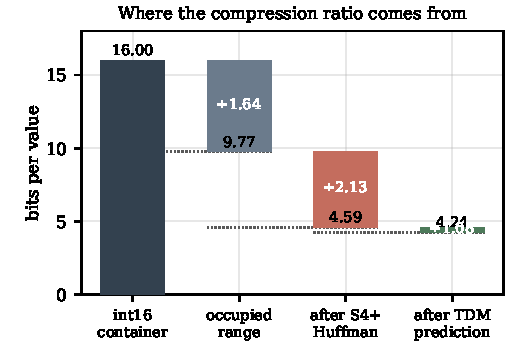
\includegraphics[width=\columnwidth]{fig_waterfall.pdf}
\caption{Decomposition of the compression ratio. Of the 16 bits in the
\texttt{int16} container, 6.2 are structurally unused because the capture sits
far below full scale; the entropy coder recovers a further factor of 2.13 from
spectral sparsity; and prediction on the corrected axis contributes the
remaining 1.08. Prediction on the uncorrected ramp axis contributes nothing at
all --- it costs 0.24 bits per value.}
\label{fig:waterfall}
\end{figure}

Coding the data with no prediction at all compresses \emph{better} than either
predictor. DRHE costs \SI{4.9}{\percent} more bits than doing nothing; LPC
costs \SI{2.6}{\percent} more. Order-0 entropy confirms the direction: the raw
FX16 codes have entropy \SI{4.094}{bits}, and the DRHE residuals have entropy
\SI{4.538}{bits}. The predictor is \emph{increasing} the entropy of the data it
is supposed to be decorrelating.

Where, then, does \num{3.489} come from? Two places, neither of which is
Doppler redundancy.

\paragraph{Unused container headroom.}
The fixed scale factor of Eq.~\eqref{eq:scale} is calibrated to a full-scale
ADC sinusoid, but the ColoRadar capture sits far below full scale: the peak raw
ADC sample is \num{914} of a possible \num{32767}. After windowing, FFT and
scaling, the peak \texttt{int16} FFT code is \num{436}. Only
$\log_2(436)+1 = 9.8$ of the \num{16} container bits ever carry information;
the remaining \num{6.2} bits are structurally zero in every sample. An entropy
coder removes them whether or not any prediction happens. This alone accounts
for a factor of $16/9.8 = 1.63$.

\paragraph{Spectral sparsity.}
The remaining $9.8 \rightarrow 4.59$ bits, a factor of \num{2.14}, is the
genuine statistical gain: a range--FFT frame is sparse, most bins are noise
close to zero, and the S4 categories concentrate accordingly. Kiem's Huffman
dictionary turns out to be well matched to this distribution --- it costs
\SI{4.586}{bits} against an order-0 entropy of \SI{4.094}{bits}, an overhead of
\SI{0.28}{bits} or \SI{6.2}{\percent}.


\begin{figure}[t]
\centering
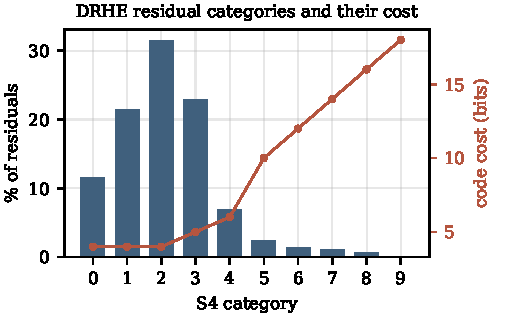
\includegraphics[width=\columnwidth]{fig_s4.pdf}
\caption{Distribution of DRHE residuals across S4 categories, with the cost of
each category from Eq.~\eqref{eq:cost}. Over \SI{87}{\percent} of residuals fall
in categories 0--3, which the fixed dictionary codes in 4 or 5 bits. The sharp
cost step above category~4 is what makes the coder sensitive to any rescaling
of the input.}
\label{fig:s4}
\end{figure}

The practical consequence is that the reported ratios are specific to this
capture's gain setting. A well-scaled capture filling the int16 container would
compress substantially less, and any comparison of these ratios against results
from a different sensor must account for that.

\subsection{The prediction axis}
\label{sec:predaxis}

The inversion in Table~\ref{tab:decomp} is not a property of the predictors ---
it is a property of the axis they were applied along. Both were predicting from
ramp $m-1$, which by Eq.~\eqref{eq:rampindex} is a different physical
transmitter eleven times in twelve. Two ramps from different transmitters
differ by the target's array steering phase, which is large and varies with
target angle. The DRHE phase model of Eq.~\eqref{eq:phasepred} assumes a
constant per-ramp phase increment; a per-ramp transmitter change makes that
increment alternate on a period-12 pattern, which a double integrator cannot
track. The LPC autocorrelations at lags 1 and 2 likewise measure the
transmitter switching pattern rather than target Doppler.

The correction is to predict from ramp $m - n_{\mathrm{Tx}}$, the previous ramp
of the \emph{same} transmitter. Table~\ref{tab:predaxis} evaluates the options
over five frames.

\begin{table}[t]
\centering
\caption{Prediction axis study, 5 frames, 4~RX, 128 bins, 192 ramps.
Prediction gain is relative to no prediction at all.}
\label{tab:predaxis}
\small
\setlength{\tabcolsep}{4pt}
\begin{tabular}{lrrr}
\toprule
Configuration & b/val & CR & gain\\
\midrule
No prediction                        & 4.586 & 3.489 & 1.000\\
DRHE lag 1 \emph{(as implemented)}   & 4.821 & 3.319 & 0.951\\
\textbf{DRHE lag $n_{\mathrm{Tx}}$}  & \textbf{4.240} & \textbf{3.774} & \textbf{1.082}\\
LPC lags 1,\,2 \emph{(as impl.)}     & 4.710 & 3.397 & 0.974\\
LPC per-TX block, $N=16$             & 6.093 & 2.626 & 0.753\\
\textbf{LPC lags $n_{\mathrm{Tx}},2n_{\mathrm{Tx}}$} & \textbf{4.269} & \textbf{3.748} & \textbf{1.074}\\
\bottomrule
\end{tabular}
\end{table}

Predicting on the true slow-time axis converts DRHE's \SI{4.9}{\percent} loss
into an \SI{8.2}{\percent} gain, and LPC's \SI{2.6}{\percent} loss into a
\SI{7.4}{\percent} gain.

The fourth row is worth noting as the obvious alternative that does not work.
Splitting the frame into twelve independent 16-ramp per-transmitter blocks and
fitting separate coefficients to each puts the predictor on the right axis, but
multiplies the coefficient side information by twelve --- from \SI{1.04}{\percent}
to \SI{12.5}{\percent} of the uncompressed frame --- and shortens each
autocorrelation estimate to 16 samples. The net effect is far worse than doing
nothing. Keeping one coefficient pair per (bin, channel, component) and simply
moving the lags to $n_{\mathrm{Tx}}$ and $2n_{\mathrm{Tx}}$ costs no extra side
information at all, which is why the last row works.

\subsection{TDM-aware implementations}
\label{sec:tdmresults}

Both corrections were implemented in HLS and put through the same verification
as the baselines. The changes are small. For DRHE the state arrays gain a
transmitter dimension, indexed by $m \bmod n_{\mathrm{Tx}}$, and the reset
condition widens from $m = 0$ to $m < n_{\mathrm{Tx}}$, since each
transmitter's history begins on its own first ramp. For LPC, both the
autocorrelation pass and the residual pass keep a ring of $2n_{\mathrm{Tx}}$
entries per (channel, bin) instead of two scalars; because the ring length is
exactly $2n_{\mathrm{Tx}}$, slot $m \bmod 2n_{\mathrm{Tx}}$ still holds the
sample from ramp $m - 2n_{\mathrm{Tx}}$ at the moment it is read, and slot
$(m + n_{\mathrm{Tx}}) \bmod 2n_{\mathrm{Tx}}$ holds ramp $m - n_{\mathrm{Tx}}$,
so nothing has to be shifted. The LPC restructure also moves the
autocorrelation accumulation out of the ingest pass into the per-bin pass,
which removes six 64-bit accumulator arrays and four history arrays entirely.

Table~\ref{tab:tdmhls} gives the measured results over the full 50-frame
dataset.

\begin{table}[t]
\centering
\caption{TDM-aware variants against their baselines, Vitis HLS C-simulation,
50 frames, 4~RX. All configurations reconstruct every sample exactly.}
\label{tab:tdmhls}
\small
\setlength{\tabcolsep}{4pt}
\begin{tabular}{lrrr}
\toprule
Design & CR & MaxDiff & $\Delta$CR\\
\midrule
DRHE, lag 1                 & 3.30987 & 0 & ---\\
\textbf{DRHE, lag $n_{\mathrm{Tx}}$} & \textbf{3.75082} & 0 & $+13.3\%$\\
LPC, lags 1,\,2             & 3.38497 & 0 & ---\\
\textbf{LPC, lags $n_{\mathrm{Tx}},2n_{\mathrm{Tx}}$} & \textbf{3.69681} & 0 & $+9.2\%$\\
\bottomrule
\end{tabular}
\end{table}


\begin{figure}[t]
\centering
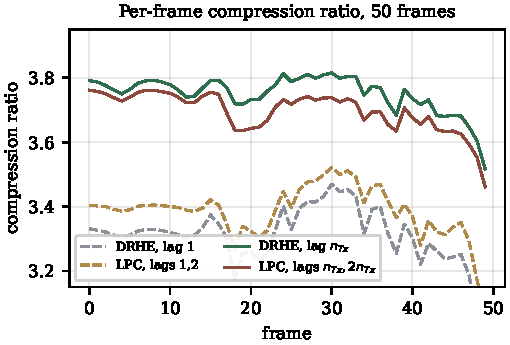
\includegraphics[width=\columnwidth]{fig_perframe.pdf}
\caption{Per-frame compression ratio over the 50-frame sequence, measured in
Vitis HLS C-simulation. The two TDM-aware variants (solid) sit consistently
above their baselines (dashed) on every frame, not merely on average. All four
configurations reconstruct every sample exactly.}
\label{fig:perframe}
\end{figure}


Table~\ref{tab:tdmsyn} gives the synthesis cost of the correction.

\begin{table}[t]
\centering
\caption{Synthesis cost of the TDM correction, \texttt{xcku5p},
\SI{100}{\mega\hertz} target. The DRHE state gains a transmitter dimension; the
LPC restructure removes the ingest accumulator arrays.}
\label{tab:tdmsyn}
\small
\setlength{\tabcolsep}{3pt}
\begin{tabular}{lrrrr}
\toprule
& \multicolumn{2}{c}{DRHE} & \multicolumn{2}{c}{LPC}\\
\cmidrule(lr){2-3}\cmidrule(lr){4-5}
Resource & lag 1 & lag $n_{\mathrm{Tx}}$ & lags 1,2 & lags $n_{\mathrm{Tx}}$,$2n_{\mathrm{Tx}}$\\
\midrule
LUT       & \num{115532} & \num{115736} & \num{80528} & \num{86298}\\
FF        & \num{57105}  & \num{57263}  & \num{17393} & \num{23154}\\
BRAM\_18K & \num{40}     & \num{80}     & \num{256}   & \num{192}\\
DSP       & \num{132}    & \num{132}    & \num{168}   & \num{156}\\
$F_{\max}$ (MHz) & 81.88 & 81.88 & 85.43 & 85.43\\
Worst loop II & 2 & 2 & 3 & \textbf{1}\\
\bottomrule
\end{tabular}
\end{table}

For DRHE the correction is close to free: \num{40} additional BRAM\_18K
(\SI{4}{\percent} of the device) buys \SI{13.3}{\percent} more compression, with
LUTs, flip-flops, DSPs and $F_{\max}$ all unchanged to within measurement
noise. The state grows by a factor $n_{\mathrm{Tx}}$ in principle, but because
the baseline was dimensioned for up to \num{1024} range bins and the corrected
version for the \num{128} actually used, the realised growth is only
$1.5\times$.


\paragraph{Latency.}
The cycle model for these designs is simply the sum over loops of trip count
times initiation interval, and it is accurate: for the baseline LPC it predicts
\num{197120} cycles against \num{197277} measured in co-simulation, an error of
\SI{0.08}{\percent}. DRHE's schedule is unchanged by the correction --- the
state indexing changes which address is read, not when --- so its frame latency
remains \num{61253} cycles. TDM-aware LPC trades its $\mathrm{II}=3$ ingest
(\num{73728} cycles) for an $\mathrm{II}=1$ ingest (\num{24576}) plus a new
correlation pass (\num{98304}), giving \num{246272} cycles, about
\SI{25}{\percent} more than the baseline. That extra pass is the price of the
deeper lags, and it is the one place where the corrected LPC is worse than the
design it replaces.

For LPC the picture is more interesting, because moving the autocorrelation out
of the ingest pass removed six 64-bit accumulator arrays and four history
arrays outright. The design uses \SI{25}{\percent} \emph{less} block RAM than
the baseline and --- more importantly --- satisfies every loop constraint at
$\mathrm{II}=1$, where the baseline was stuck at $\mathrm{II}=3$ on accumulator
port pressure. The cost is \SI{7}{\percent} more LUTs and \SI{33}{\percent}
more flip-flops for the $2n_{\mathrm{Tx}}$-entry rings, and one additional pass
over the frame buffer.

The measured \num{3.75082} for TDM-aware DRHE agrees with the \num{3.774}
predicted by the five-frame MATLAB study of Table~\ref{tab:predaxis} to within
the frame-to-frame spread, which is the expected cross-check.

\section{Discussion}
\label{sec:discussion}

\subsection{Comparison with the reference design}

Direct comparison against the reference DRHE implementation~\cite{kiem2023} is
informative but not like-for-like: different device, different radar, different
dataset and different detection pipeline. Two corrections are needed before any
comparison at all.

\paragraph{Device size.}
The \texttt{xcku5p} used here is roughly three times the ZU3EG of the reference
design (\num{216960} versus \num{70560} LUTs). Percentage utilisations are
therefore not comparable, and only absolute counts mean anything. In absolute
terms this DRHE implementation uses \num{2.5}$\times$ the LUTs of the
reference.

\paragraph{Throughput units.}
The reference reports \SI{11.92}{Gbit\per\second} at \SI{100}{\mega\hertz}.
Taken as decimal gigabits that is \num{119.2} bits per cycle on a 128-bit
input, which is an awkward number with no architectural interpretation. Taken
as \emph{gibibits}, $11.92 \times 2^{30} / 10^{8} = 127.99$ bits per cycle ---
exactly \num{128}, the full width of the AXI4-Stream input, at
$\mathrm{II}=1$. The reference figure is therefore in binary units, and its
decimal equivalent is \SI{12.80}{Gbit\per\second}. Any comparison against
\num{11.92} understates the gap by \SI{7.4}{\percent}.

With that correction, Table~\ref{tab:throughput} gives the honest comparison.

\begin{table}[t]
\centering
\caption{Throughput comparison. The reference column restates the published
figure in decimal units.}
\label{tab:throughput}
\small
\setlength{\tabcolsep}{4pt}
\begin{tabular}{lrrr}
\toprule
& DRHE & LPC & Ref.~\cite{kiem2023}\\
\midrule
Effective II            & 2   & 3   & 1\\
bits/cycle              & 51.4 & 15.9 & 128.0\\
Throughput @\SI{100}{\mega\hertz} & \SI{5.14}{Gbit/s} & \SI{1.60}{Gbit/s} & \SI{12.80}{Gbit/s}\\
Pipeline latency        & \SI{580}{\nano\second} & --- & \SI{230}{\nano\second}\\
\bottomrule
\end{tabular}
\end{table}

The gap is structural rather than mysterious. The reference achieves
$\mathrm{II}=1$; this DRHE achieves $\mathrm{II}=2$ on a BRAM port conflict,
and loses a further \SI{20}{\percent} to per-ramp pipeline drain. Fixing the
port conflict --- by partitioning the state arrays cyclically on the bin
dimension, or by hoisting the first-ramp reset out of the pipelined loop ---
would bring this design to \SI{11}{} to \SI{12}{Gbit\per\second}, in line with
the reference. LPC's $\mathrm{II}=3$ ingest and its scalar residual pass are
similarly addressable: unrolling the channel dimension in the residual pass
would cut it from \num{98304} to about \num{24576} cycles, and fixing the
ingest accumulator pressure would take \num{73728} cycles to \num{24576}. Both
together would put LPC within \SI{20}{\percent} of DRHE without touching the
algorithm. The division is emphatically not the bottleneck: it runs \num{1024}
times per frame and contributes \num{512} of \num{197277} cycles.

\subsection{DRHE or LPC?}

On compression ratio alone the two are close, and after the TDM correction DRHE
is ahead (\num{3.751} versus \num{3.697}). On logic LPC is clearly cheaper:
\SI{30}{\percent} fewer LUTs and \SI{70}{\percent} fewer flip-flops, because
its per-sample work is two fixed-point multiply-accumulates rather than four
floating-point transcendentals. On memory and latency DRHE is clearly better:
it needs no frame buffer at all, where LPC needs \SI{3.1}{\mebi bit} and a full
frame of latency before it can emit its first bit.

For the use case that motivates this work --- a compression IP sitting between
the range FFT and the memory bus in a streaming sensor front end --- latency and
streaming behaviour outrank a few percent of ratio, and DRHE is the better
choice. Where a frame of latency is acceptable and BRAM is plentiful, LPC's
logic saving is real.

The result that did not survive contact with measurement is the prior
expectation that LPC's division would make it the expensive design. It does
not. The expensive operations in this problem are \texttt{atan2} and the
sine/cosine pair, not division.

\subsection{Threats to validity}

Several limitations bound how far these results generalise, and are stated
plainly rather than buried.

\begin{itemize}\itemsep2pt
\item \textbf{The compression ratios are capture-specific.} As
  Section~\ref{sec:decomp} shows, most of the ratio comes from an under-filled
  \texttt{int16} container. A capture with \SI{6}{dB} more gain would compress
  measurably less.

\item \textbf{The detection metrics do not measure compression.} All three
  lossless schemes share identical detection metrics with FX16 by construction.
  What the metrics measure is the cost of the FX16 quantisation step.

\item \textbf{FP\% is a false discovery rate.} It normalises by test
  detections, not by true negatives. It is a legitimate metric but not the one
  its conventional name denotes.

\item \textbf{Detection matching has no positional tolerance.} A target
  displaced by one range--Doppler cell is scored as both a miss and a false
  discovery. This inflates both rates relative to a matched-detection
  criterion.

\item \textbf{The detection threshold is a free parameter.} The mean of the
  lowest \SI{75}{\percent} of magnitudes plus \SI{15}{\decibel} is not swept,
  and the detection metrics are sensitive to it.

\item \textbf{Channel count differs between phases.} The MATLAB benchmark of
  Table~\ref{tab:phase1} uses all 16 receive channels; the hardware path uses
  4, which is the AXI4-Stream width. Compression ratios between the two are
  therefore compared through a like-for-like MATLAB helper rather than
  directly.

\item \textbf{All hardware numbers are pre-implementation estimates.}
  $F_{\max}$, resources and latency come from HLS synthesis and RTL
  co-simulation, not from place-and-route or silicon. Phase~4 remains
  outstanding.

\item \textbf{Two source citations required correction.} The BAQ baseline is
  properly attributed to Kwok and Johnson~\cite{kwok1989baq} --- IEEE~TGRS
  vol.~27, no.~4, pp.~375--383, 1989, on \emph{synthetic} aperture radar. An
  earlier draft of this work carried an author name, title and page range that
  do not correspond to any such paper. The ColoRadar citation is likewise
  vol.~41, no.~4, pp.~351--360 (2022), not vol.~40 (2021). Both are corrected
  in the bibliography here.

\item \textbf{$n_{\mathrm{Tx}} = 12$ is assumed constant.} The TDM-aware
  variants take the transmitter count as a runtime parameter but assume a fixed
  TDM pattern. A radar that changes its MIMO schedule mid-stream would need the
  parameter re-loaded between frames.
\end{itemize}

\section{Conclusions}
\label{sec:conclusion}

Two lossless compressors for radar range--FFT data were implemented in Vitis
HLS for a Kintex UltraScale+ device, verified bit-exactly against a MATLAB
golden reference over 50 frames of real cascaded MIMO radar data, and
characterised by RTL co-simulation. Both reconstruct every sample of every
frame exactly.

The main result is a correction. Applying either predictor along the raw ramp
axis of a TDM-MIMO cascade is wrong, because that axis interleaves
transmitters: the predictors were performing \emph{worse} than no prediction at
all, and the compression ratios being reported were almost entirely the work of
the entropy coder on an under-filled \texttt{int16} container. Moving the
prediction to lag $n_{\mathrm{Tx}}$ puts it on the true slow-time axis and
recovers the gain the algorithms were designed to deliver: measured compression
rises from \num{3.310} to \num{3.751} for DRHE and from \num{3.385} to
\num{3.697} for LPC, in both cases with reconstruction still exact. For DRHE
the cost is $n_{\mathrm{Tx}}$ copies of the predictor state --- \num{40}
additional BRAM\_18K, or \SI{4}{\percent} of the device --- with logic and
$F_{\max}$ essentially unchanged.

Two implementation defects were found and fixed: a residual of $-32768$ that
the S4/APPEND code cannot represent and which aliased silently onto $+32767$,
resolved by saturation combined with closed-loop prediction so that encoder and
decoder cannot diverge; and a 128-bit to single-precision conversion in the
Yule--Walker solver that returned zero above $2^{64}$, resolved by normalising
all operands through a common arithmetic shift. Neither was visible on real
data; both were caught by synthetic edge cases, which is an argument for
keeping such a suite alongside dataset-driven verification.

Three quantitative claims in the surrounding literature were checked and one
required correction: the widely quoted \SI{11.92}{Gbit\per\second} is in
gibibits, and equals \SI{12.80}{Gbit\per\second} decimal, or exactly
\num{128} bits per cycle at \SI{100}{\mega\hertz}.

\paragraph{Future work.}
The immediate items are the two identified throughput fixes --- resolving
DRHE's BRAM port conflict to reach $\mathrm{II}=1$, and unrolling LPC's
residual pass --- followed by place-and-route and on-silicon measurement to
replace the estimates in Table~\ref{tab:resources}. Beyond that, the
decomposition of Section~\ref{sec:decomp} suggests the most valuable single
change would be to make the FX16 scale factor adaptive per frame, which would
both use the container properly and make the reported ratios reflect prediction
performance rather than capture gain.

\begin{thebibliography}{9}
\small
\bibitem{kramer2021coloradar}
A.~Kramer, K.~Harlow, C.~Williams and C.~Heckman,
``ColoRadar: The direct 3D millimeter wave radar dataset,''
\emph{The International Journal of Robotics Research}, vol.~41, no.~4,
pp.~351--360, 2022.

\bibitem{kiem2023}
L.~Kiem, ``Design and implementation of data compression methods for SoC-based
radar systems,'' Master's thesis, Institute of Technical Informatics,
Graz University of Technology, Graz, Austria, May 2025.

\bibitem{kwok1989baq}
R.~Kwok and W.~T.~K. Johnson, ``Block adaptive quantization of Magellan SAR
data,'' \emph{IEEE Transactions on Geoscience and Remote Sensing}, vol.~27,
no.~4, pp.~375--383, Jul.~1989.

\end{thebibliography}

\balance
\end{document}
